\subsection*{Modelización 1}

Jugando con un perro, se le arroja una pelota que recorre 20 metros, cuya altura sigue la función $y = \frac{-1}{40}x^2+\frac{2}{5}x+2$. En este modelo, la altura es la variable dependiente y la distancia la variable independiente. 

Gráficamente:

\begin{align*}
	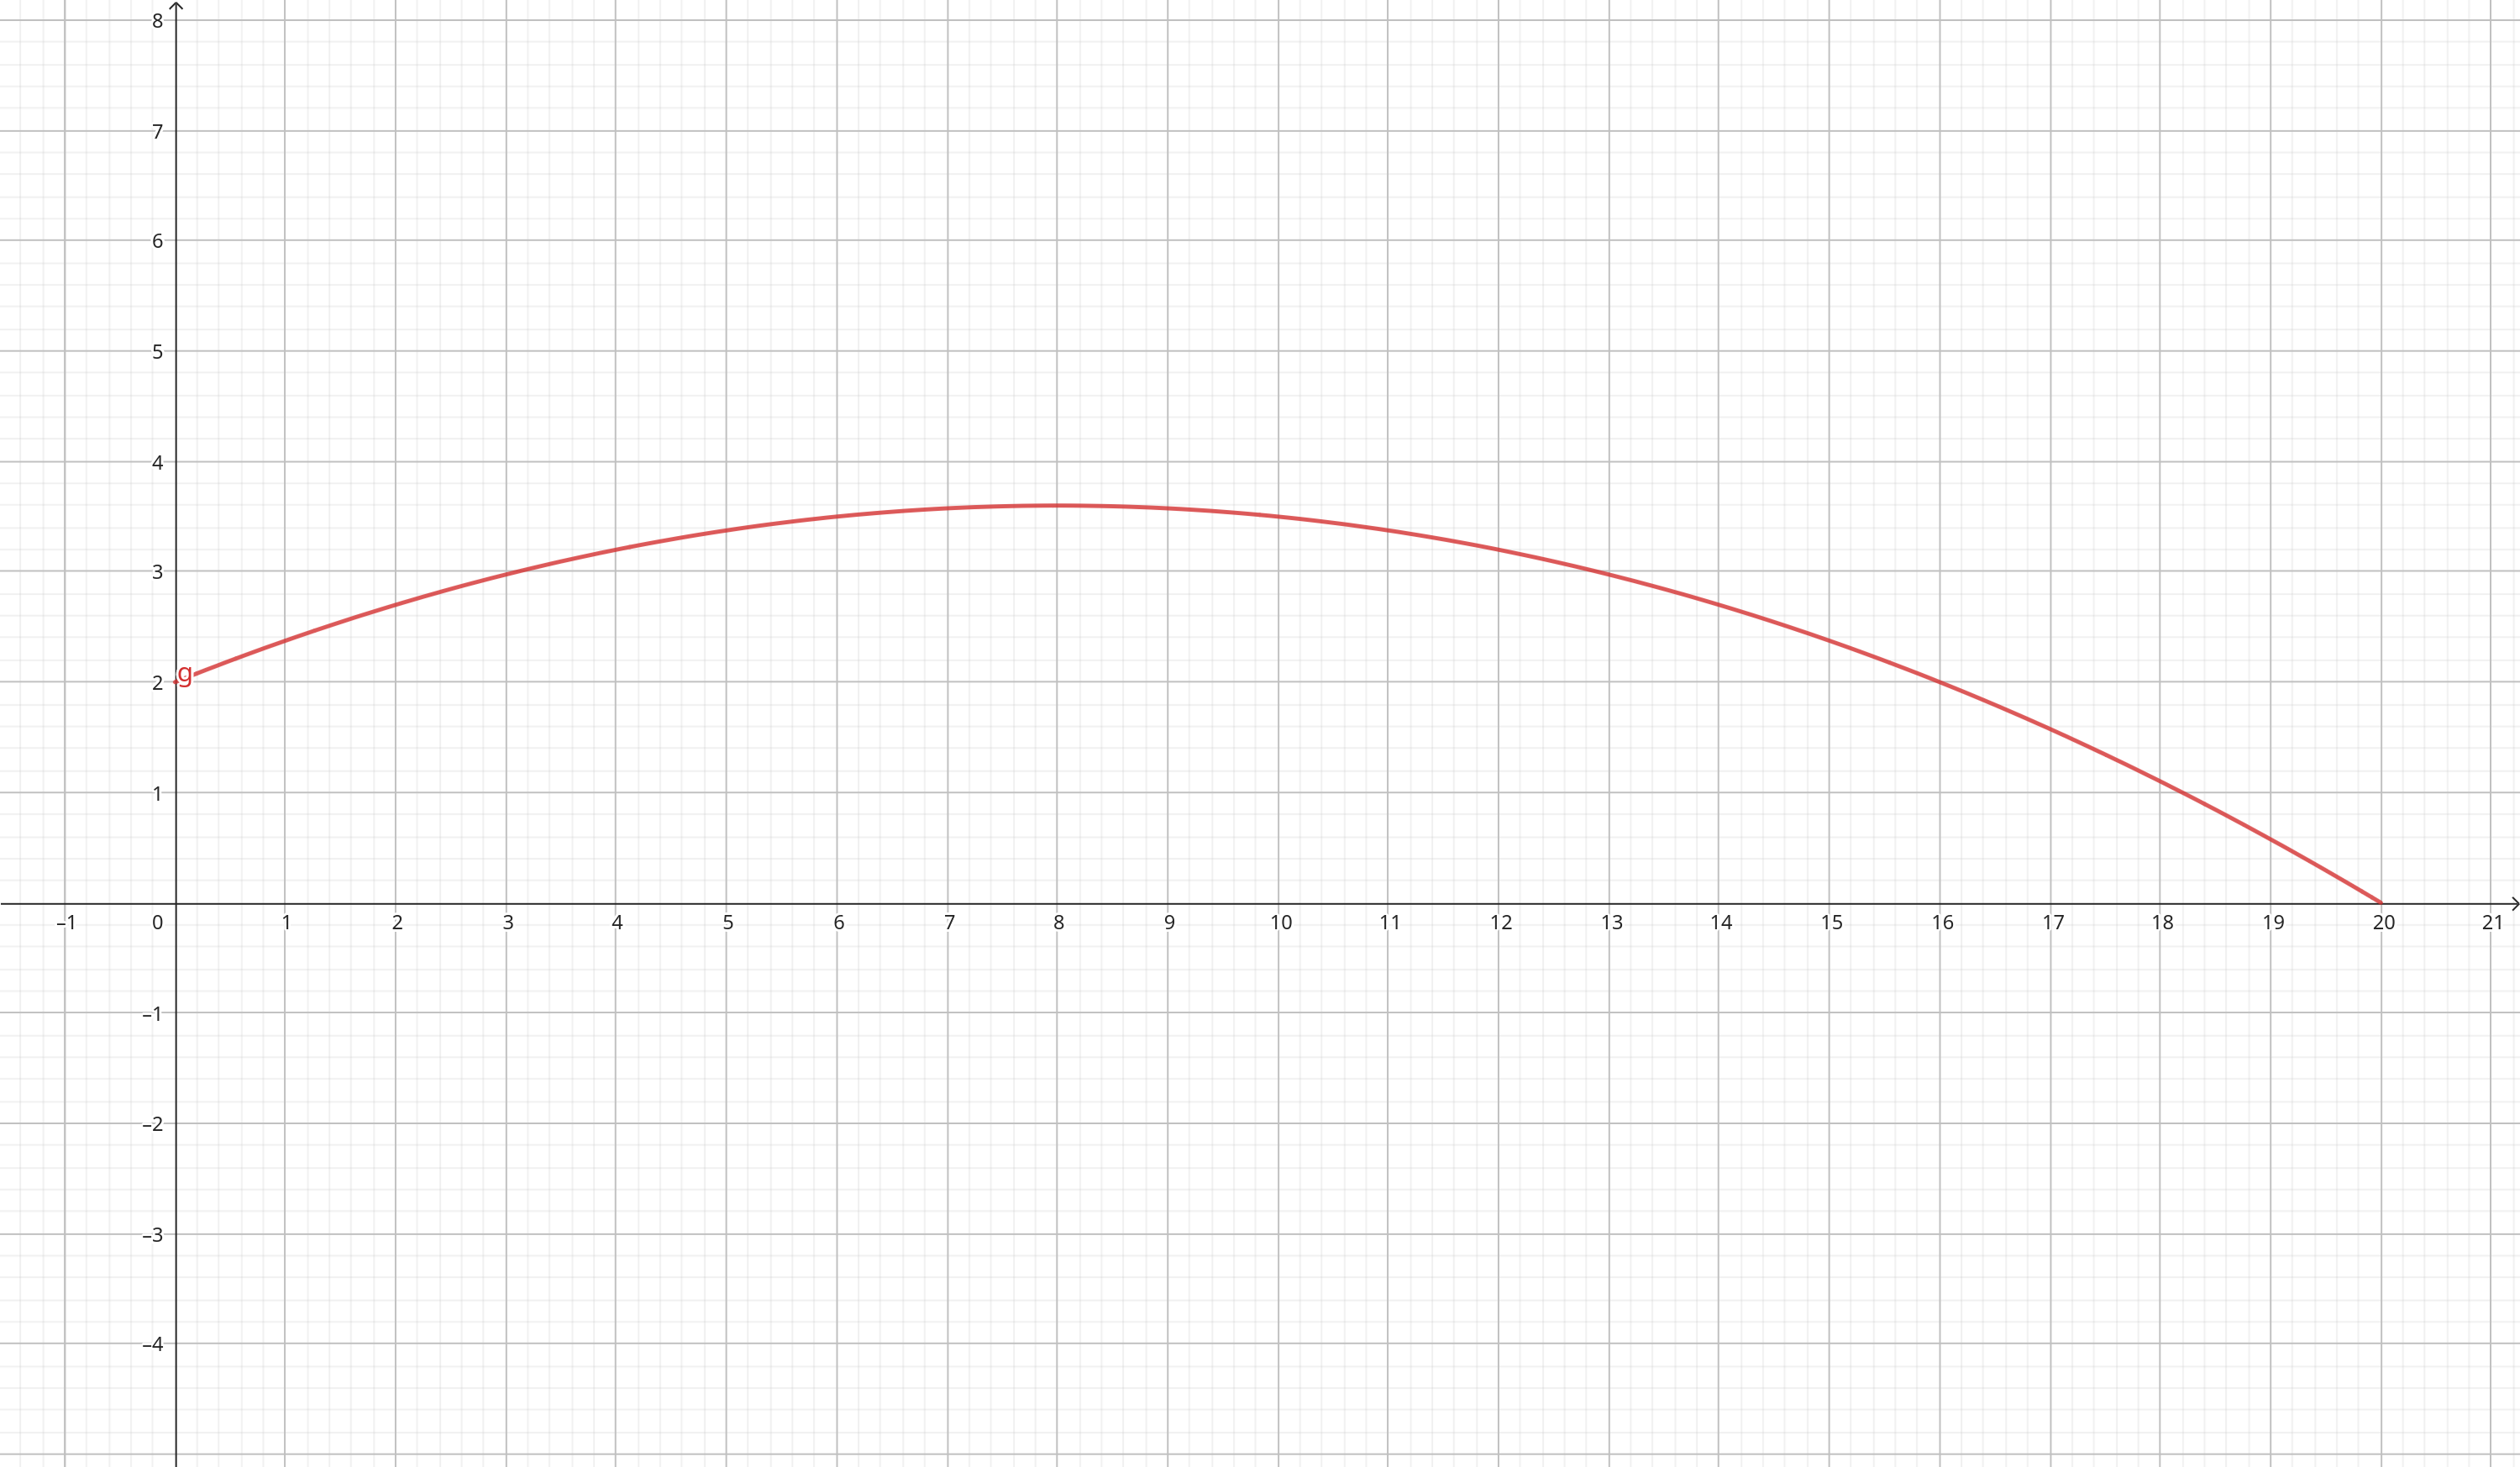
\includegraphics[scale=.7]{02/actividad1/img/modelo1.png}
\end{align*}

Su dominio es $D = [0,20]$ y su conjunto imagen es $I = [0, 3,6]$.
